\section{Rich Pictures}\label{sec:rich-pictures}

The authors decided to create rich pictures about the problem faced by Nova to get a better understanding
of the problem cafe Nova is currently facing for their current operation.

\begin{figure}
    \centering
    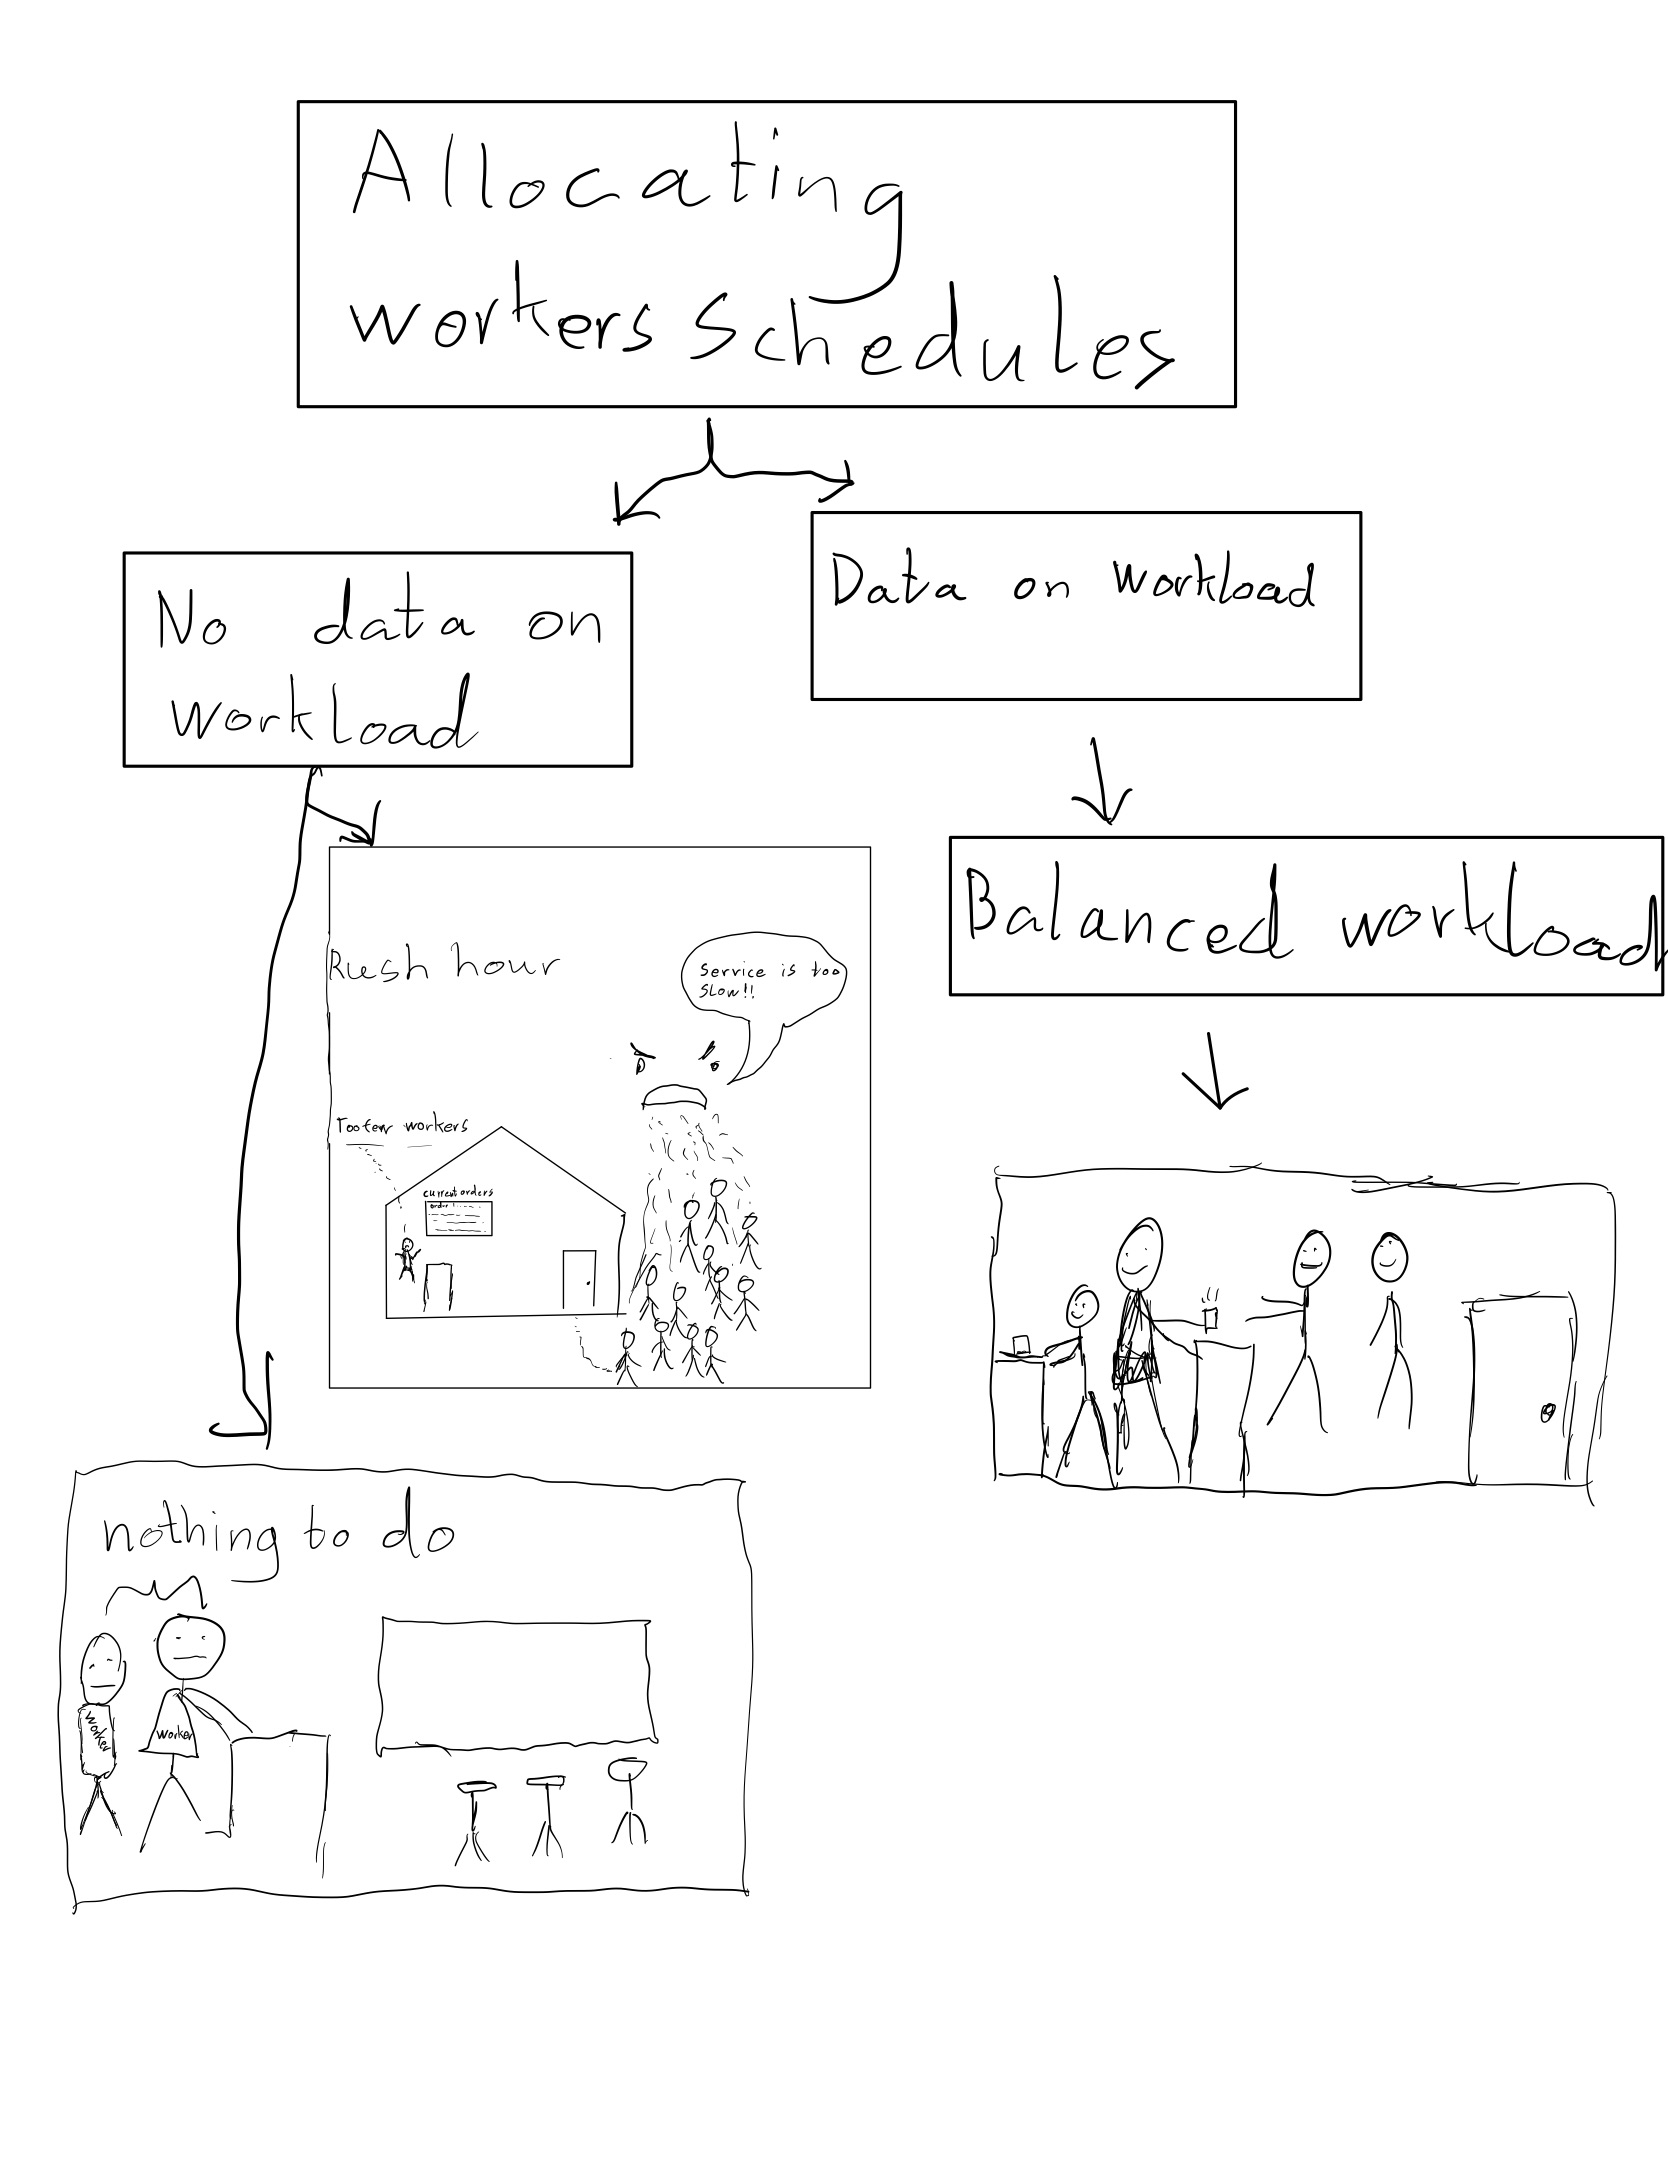
\includegraphics{rich-picture-problem}
    \caption{Rich picture of cafe Novas problems.}\label{fig:rich-picture-problem}
\end{figure}

As seen in figure~\ref{fig:rich-picture-problem}, one of the key identified ussues the Nova cafe has is planning for
customer droughts and rush hours.

Currently, planning happens by the experience of the manager, depending on their skills, they can either succeed creating
the correct schedule or not.
In practice, guessing the customer flow is challenging, and if mistakes are made, there exist two worst case scenarios.
One would be too many workers for a given hour, this results in workers not having enough tasks to do, and is not
optimal or viable from the café's perspective.
The other possibility is too few workers during a rush hour, this is bad because it leads to degraded service for the
customer, and therefore a bad experience.
Worst case this can turn away new customers and is also something Nova will want to avoid.

The agreed upon solution would give the café a way to get, and visualize data around the customer flow during
opening hours, this is visualized in figure~\ref{fig:rich-picture-solution}.

\begin{figure}
    \centering
    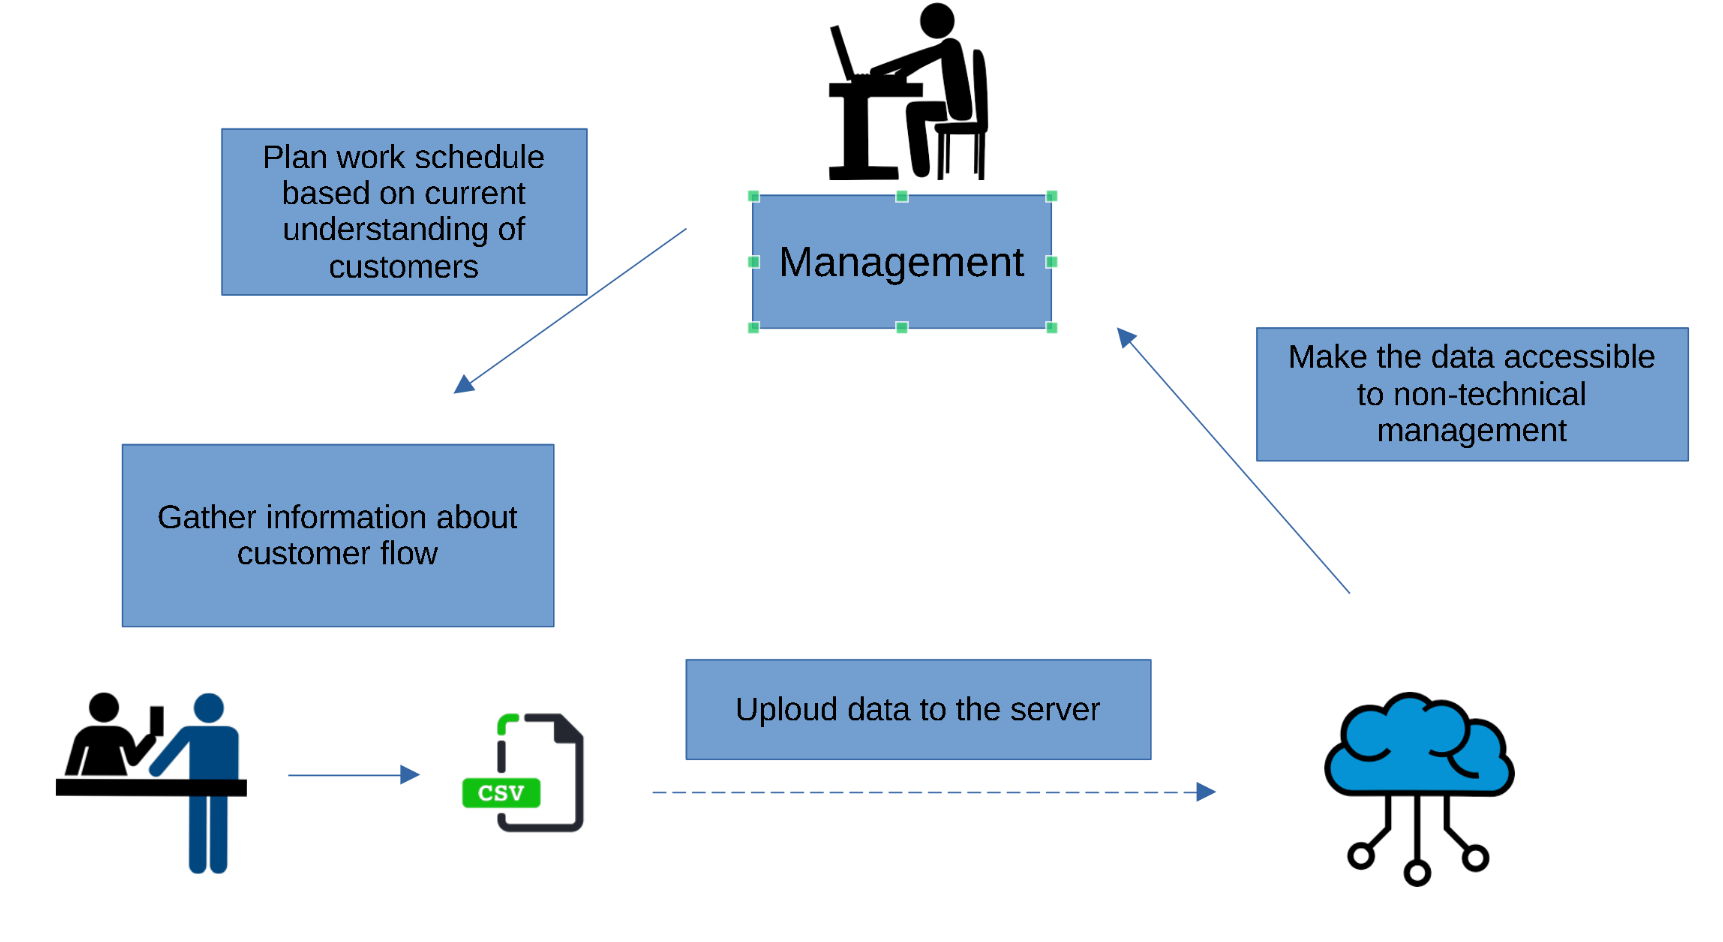
\includegraphics{rich-picture-solution}
    \caption{Rich picture of the planned solution to Novas problems.}\label{fig:rich-picture-solution}
\end{figure}

The goal of this project is then to give café Nova a product that helps them understand their customer flow.
How this solution will look and work will be discussed in later sections.
